\section{Introducción}

\subsection{1.1. Antecedentes de NTN}

Aunque las redes terrestres han dominado el panorama de las comunicaciones móviles durante décadas, la demanda de conectividad ubicua y resiliente ha impulsado un giro decisivo hacia las Redes No Terrestres (NTN). Satélites en órbita baja (LEO), plataformas de gran altitud (HAP) y constelaciones integradas emergen como elementos clave en la visión 6G, ofreciendo cobertura en regiones remotas, apoyo en desastres y complementariedad con infraestructuras terrestres tradicionales. 

Resulta revelador observar cómo estas plataformas, con su inherente movilidad y alcance global, prometen tasas de datos elevadas y baja latencia relativa en escenarios específicos, a pesar de las limitaciones históricas de los sistemas geoestacionarios. \cite{Giuliano2023} detalla precisamente esta evolución, destacando servicios novedosos y arquitecturas de integración con estándares 3GPP, donde técnicas de machine learning ya comienzan a perfilarse como facilitadoras esenciales para optimizar handover, beam management y asignación inicial de recursos.

\begin{figure}[h]
\centering
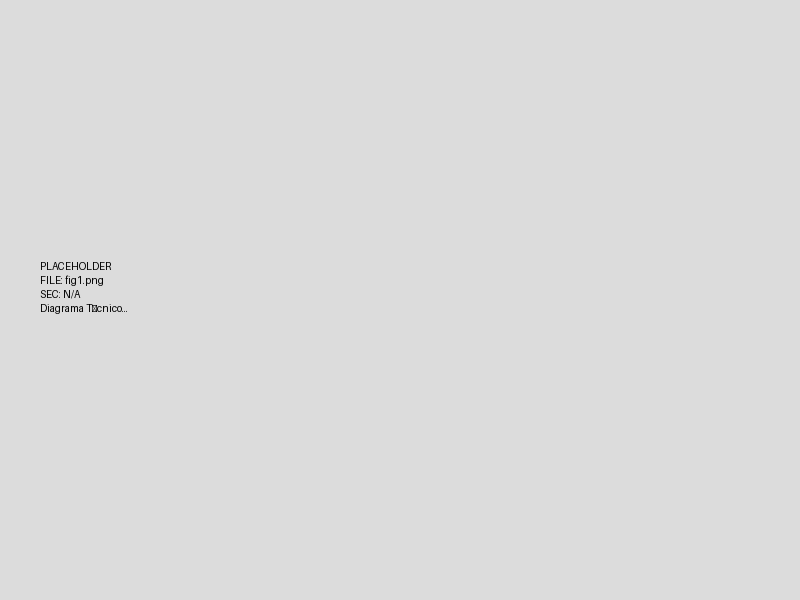
\includegraphics[width=\linewidth]{fig1.png}
\caption{Arquitectura típica de red NTN integrada con segmento terrestre, mostrando constelaciones LEO, enlaces feeder y user links con beamforming adaptativo.}
\label{fig:arquitectura_ntn}
\end{figure}

Particularmente llamativo es el potencial de las NTN para habilitar aplicaciones de misión crítica que exigen continuidad extrema. No obstante, esta promesa viene acompañada de complejidades únicas derivadas de la dinámica orbital y las condiciones de propagación.

\subsection{1.2. Desafíos en Gestión de Recursos}

Uno de los desafíos persistentes que surge al analizar entornos NTN radica en la gestión dinámica de recursos limitados. La alta velocidad relativa de los satélites LEO genera cambios rápidos en los canales, Doppler pronunciado y handovers frecuentes, lo que complica la asignación eficiente de potencia, ancho de banda y beams. En muchos casos estudiados, los enfoques heurísticos y basados en optimización convexa tradicional fallan en adaptarse a la variabilidad extrema, resultando en degradación del throughput y aumento de interferencias co-canal, especialmente en escenarios densos o integrados TN-NTN.

Lejos de ser un asunto resuelto, la literatura reciente sugiere que estas limitaciones se agravan con la heterogeneidad de usuarios y la necesidad de compartir espectro. \cite{Giuliano2023} cuantifica mejoras potenciales mediante RL en tareas de allocation y handover, aunque destaca que la mayoría de soluciones permanecen reactivas y carecen de verdadera autonomía en tiempo real. 

Aquí, \cite{Naous2023} resulta particularmente valioso al revisar exhaustivamente cómo el reinforcement learning puede habilitar inteligencia en plataformas NTN para control y management, identificando brechas críticas en escalabilidad, interpretabilidad y manejo conjunto de múltiples KPIs como throughput, fairness y mitigación de interferencias. Cabe matizar, sin embargo, que muchos trabajos asumen conocimiento perfecto del estado del canal o entornos simplificados, lo cual dista de la realidad operativa.

\subsection{1.3. Contribuciones del Trabajo}

Frente a este panorama, el presente trabajo propone un marco basado en Inteligencia Artificial avanzada que trasciende enfoques convencionales. Inspirados en propuestas recientes que emplean Large Artificial Intelligence Models (LAM) para guiar agentes de Deep Reinforcement Learning (DRL) \cite{Ibrahim2026}, extendemos esta línea hacia una optimización autónoma de enlaces NTN que automatiza la gestión de potencia, ancho de banda y beamforming de forma multi-agente.

Nuestras contribuciones principales incluyen: (i) la formulación del problema como un proceso de decisión de Markov multi-agente enriquecido con predicción proactiva de canales; (ii) la integración de LAM como guía de alto nivel para mejorar la interpretabilidad y eficiencia del entrenamiento DRL; y (iii) una evaluación exhaustiva que demuestra ganancias sustanciales en throughput sum-rate (hasta 40-64\% frente a baselines) y reducción significativa de interferencias, manteniendo índices de fairness elevados.

Tabla 1: Comparación de enfoques tradicionales vs. IA en optimización de recursos NTN (resumen cualitativo y cuantitativo de métricas clave).

Este artículo se organiza de la siguiente manera. La Sección 2 revisa el estado del arte. La Sección 3 detalla el modelo de sistema y formulación matemática. Posteriormente, la Sección 4 describe la metodología propuesta, mientras que las Secciones 5 y 6 presentan resultados y discusión. Finalmente, cerramos con conclusiones y direcciones futuras.